\documentclass{article}
\usepackage{graphicx} % Required for inserting images
\usepackage{minted}

\title{Compte rendu Test}
\author{Timothé Boyer}
\date{November 2023}


\begin{document}

\maketitle

\section{Tests}
Dans cette partie du compte rendu nous nous interesserons au test realisé sur les différentes partie de notre programme.
\\
De plus beaucoup de test ont été fait en utilisant le programme lorsque l'on jouait contre des IA
\subsection{Tests de conception du jeu d'échec}
Nous avons réalisé des tests sur les différents programme qui permettent au jeu d'échec de fonctionner.

Pour tester le bon fonctionnement du jeu nous avons utiliser la fonctionalité nous permettant d'importer des sauvegardes car ainsi on peut tester des situations précise et voir si tous fonctionne comme prévu.
\\
On crée donc une fonction dont le but est de créer des parties à partir du nom du fichier de test. Ce qui nous permet de ranger les tests dans différents les différents dossiers dédiés à chaque test.

\subsubsection{Tests de la classe pièce}
Pour tester les pièces nous avons d'abord testé la méthode coups\_possible pour chacune des pièces existantes. Pour ça nous avons d'abords créer une situations avec la pièces que que l'on veut tester. On note à la main toutes les cases accessibles par cette pièces et on verifie si la méthode coups\_possible de cette pièces renvoit la même liste de coups.

\begin{minted}[mathescape,
    linenos,
    numbersep=5pt,
    gobble=2,
    frame=lines,
    framesep=2mm]{python}

    #déplacement des pièces
    def test_deplacement_pion():
        partie=init_partie_test("test_deplacement_pion")
        partie.pieces[1][1].premier_coup=False
        assert partie.pieces[1][0].coups_possibles(partie)==[(3, 4), (4, 4)]
        assert partie.pieces[1][1].coups_possibles(partie)==[]
        assert partie.pieces[1][2].coups_possibles(partie)==[(1, 2), (1, 3)]
    
    def test_deplacement_fou():
        partie=init_partie_test("test_deplacement_fou")
        assert partie.pieces[1][0].coups_possibles(partie)==[(5,5),(6,6),(7,7),(5,3),(3,3),(2,2),
        (1,1),(3,5),(2,6),(1,7)]
                
    def test_deplacement_tour():
        partie=init_partie_test("test_deplacement_tour")
        assert partie.pieces[0][1].coups_possibles(partie)==[(5, 4), (6, 4), (7, 4), (4, 5), 
        (3, 4), (2, 4), (1, 4), (4, 3), (4, 2), (4, 1)]
    
    
    def test_deplacement_reine():
        partie=init_partie_test("test_deplacement_reine")
        assert partie.pieces[0][0].coups_possibles(partie)==[(5, 5), (6, 6), (5, 3), (3, 3), 
        (2, 2), (1, 1), (0, 0), (3, 5), (2, 6), (1, 7), 
        (5, 4), (6, 4), (7, 4), (4, 5), (4, 6), (4, 7), (3, 4), 
        (2, 4), (4, 3)]
    
    def test_deplacement_cavalier():   
        partie=init_partie_test("test_deplacement_cavalier")
        assert partie.pieces[1][1].coups_possibles(partie)==[(5, 5), (3, 5), (2, 4), (2, 2), 
        (3, 1), (5, 1), (6, 2)]
\end{minted}

\\
Il faut ensuite vérifier si il est bien pas possible de déplacer une pièce en mettant le roi en echec. Cette fonctionalité correspond a la méthode coups\_legaux de la classe Pièce. Pour vérifier si ça marche on fait donc un plateau avec une pièce qui est clouée (si elle bouge le roi est en echec) et on vérifie que elle n'ai pas de coups légaux.

\begin{minted}[mathescape,
    linenos,
    numbersep=5pt,
    gobble=2,
    frame=lines,
    framesep=2mm]{python}

    def test_coups_legaux():
        partie=init_partie_test("test_coups_legaux")
        assert partie.pieces[1][0].coups_possibles(partie)==[(5, 3), (3, 3), (2, 2), (2, 0), 
        (6, 0), (6, 2)]
        assert partie.pieces[1][0].coups_legaux(partie)==[]

\end{minted}
\paragraph{Validation des tests}
\begin{center}
    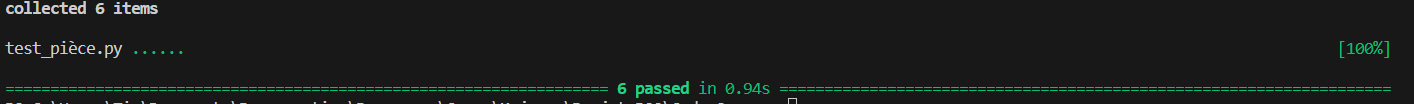
\includegraphics{pytest_piece.png}
\end{center}
\subsubsection{Tests EtatJeu}
\paragraph{Tests des echec}
\\
Nous avons fait différents tests pour voir si les méthodes echec et echec\_et\_mat fonctionne correctement. Pour ça on créer 3 situations:
\begin{itemize}
    \item Une avec le joueur qui doit jouer en echec
    \item Une sans echec et donc sans mat
    \item Une autre ou le joueur qui doit jouer est en echec et mat
\end{itemize}
\begin{minted}[mathescape,
    linenos,
    numbersep=5pt,
    gobble=2,
    frame=lines,
    framesep=2mm]{python}

    def test_pat():
        #1er situation de nulle, il n'y a pas d'echec et mat et aucun coups n'est possible
        partie=init_partie_test("pat_1")
        assert partie.nulle()
        #2nd situation de nulle, seul les rois bougent
        partie=init_partie_test("pat_2")
        partie.pieces[1][0].odometre=40
        assert partie.nulle()
        
    def test_echec():
        partie=init_partie_test("avec_echec")
        assert partie.echec()
        partie=init_partie_test("sans_echec")
        assert not partie.echec()
    
    def test_mat():
        partie=init_partie_test("avec_mat")
        assert partie.echec_et_mat()
        partie=init_partie_test("sans_mat")
        assert not partie.echec_et_mat()

\end{minted}

\paragraph{Tests de la valeur} 
Pour tester le calcul de la valeur on a créer des plateau simple ou il possible de calculer à la main facilement la valeur du plateau.

\begin{minted}[mathescape,
    linenos,
    numbersep=5pt,
    gobble=2,
    frame=lines,
    framesep=2mm]{python}
    #Test valeur:
    def test_valeur():
        #Test de situation finale
        partie=init_partie_test("avec_mat")
        assert partie.calcul_valeur()==-1000
        partie=init_partie_test("pat_1")
        assert partie.calcul_valeur()==0
        #Test centre et sous centre
        partie=init_partie_test("controle_centre_et_ss_centre")
        assert partie.calcul_valeur()==0.4
        #Test pions allignés
        partie=init_partie_test("pions_allignes")
        assert partie.calcul_valeur()==-0.1
\end{minted}
\paragraph{Validation des tests}
\begin{center}
    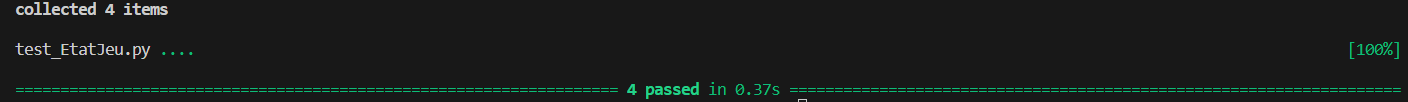
\includegraphics{pytest_EtatJeu.png}
\end{center}
\subsection{Tests IA}
Nous avons aussi testé l'IA sur plusieurs points. 

\subsubsection{Tests d'existence des coups}
Pour cette partie, on regarde si l'IA pour différentes profondeurs fait bien des coups existants.

\begin{minted}[mathescape,
    linenos,
    numbersep=5pt,
    gobble=2,
    frame=lines,
    framesep=2mm]{python}

    # Test jouer un coup
    # Test IA aléatoire (niveau == 0)
    def test_IA_0():
        partie, bot1, bot2 = initialiser_plateau_bots(profondeur_blanc=0, profondeur_noir=0)
        # Blanc
        coup = bot1.jouer_coup(partie)
        assert coup[0] in partie.mouvements(True).keys()
        assert coup[1] in partie.mouvements(True)[coup[0]]
        partie.deplacer_piece(coup[0], coup[1])
        # Noir
        coup = bot2.jouer_coup(partie)
        assert coup[0] in partie.mouvements(False).keys()
        assert coup[1] in partie.mouvements(False)[coup[0]]
    
    def test_minimax_profondeur_1():
        partie, bot1, bot2 = initialiser_plateau_bots(profondeur_blanc=1, profondeur_noir=1)
        # Blanc
        coup = bot1.jouer_coup(partie)
        assert coup[0] in partie.mouvements(True).keys()
        assert coup[1] in partie.mouvements(True)[coup[0]]
        partie.deplacer_piece(coup[0], coup[1])
        # Noir
        coup = bot2.jouer_coup(partie)
        assert coup[0] in partie.mouvements(False).keys()
        assert coup[1] in partie.mouvements(False)[coup[0]]
    
    def test_minimax_profondeur_2():
        partie, bot1, bot2 = initialiser_plateau_bots(profondeur_blanc=2, profondeur_noir=2)
        # Blanc
        coup = bot1.jouer_coup(partie)
        assert coup[0] in partie.mouvements(True).keys()
        assert coup[1] in partie.mouvements(True)[coup[0]]
        partie.deplacer_piece(coup[0], coup[1])
        # Noir
        coup = bot2.jouer_coup(partie)
        assert coup[0] in partie.mouvements(False).keys()
        assert coup[1] in partie.mouvements(False)[coup[0]]
        
        
    def test_minimax_profondeur_3():
        partie, bot1, bot2 = initialiser_plateau_bots(profondeur_blanc=3, profondeur_noir=3)
        # Blanc
        coup = bot1.jouer_coup(partie)
        assert coup[0] in partie.mouvements(True).keys()
        assert coup[1] in partie.mouvements(True)[coup[0]]
        partie.deplacer_piece(coup[0], coup[1])
        # Noir
        coup = bot2.jouer_coup(partie)
        assert coup[0] in partie.mouvements(False).keys()
        assert coup[1] in partie.mouvements(False)[coup[0]]
        
    # Test si minimax ne se suicide pas 
    def test_pas_de_suicide():
        # Initialisation d'un plateau où les blancs peuvent être mis en échec et mat en 1, on vérifie qu'il ne joue pas un coup qui le ferait perdre
        partie, bot_blanc, bot_noir = initialiser_plateau_bots("Sauvegarde_Test_IA\\suicide")
        coup = bot_blanc.jouer_coup(partie)
        partie.deplacer_piece(coup[0], coup[1])
        coup = bot_noir.jouer_coup(partie)
        partie.deplacer_piece(coup[0], coup[1])
        assert not partie.echec_et_mat()    
\end{minted}

\subsubsection{Tests de cohérence}
On vérifie maintenant si les algorithmes alphabeta et minimax proposent le même coup.

\begin{minted}[mathescape,
    linenos,
    numbersep=5pt,
    gobble=2,
    frame=lines,
    framesep=2mm]{python}

    # Test si minimax et alphabeta jouent le même coup (profondeur 2)
    def test_alphabeta():
        plateaux = ["Sauvegarde_Test_IA\\Plateau_base","Sauvegarde_Test_IA\\suicide"]
        for plateau in plateaux:
            partie_ab, bot_blanc_ab, bot_noir_ab = initialiser_plateau_bots(plateau)
            partie_mm, bot_blanc_mm, bot_noir_mm = initialiser_plateau_bots(plateau)
            bot_blanc_mm.algo = "minimax"
            bot_noir_mm.algo = "minimax"
            if partie_ab.trait:
                assert bot_blanc_mm.jouer_coup(partie_ab) == bot_blanc_ab.jouer_coup(partie_ab)
                print(bot_blanc_mm.jouer_coup(partie_ab) == bot_blanc_ab.jouer_coup(partie_ab))
            else : 
                assert bot_noir_mm.jouer_coup(partie_ab) == bot_noir_ab.jouer_coup(partie_ab)
                print(bot_noir_mm.jouer_coup(partie_ab) == bot_noir_ab.jouer_coup(partie_ab))

\end{minted}

\subsubsection{Tests de durées}
Nous avons aussi vérifié si l'algorithme alphabeta était plus optimisé que minimax et que donc le temps d'exécution de chaque coup était plus court pour alphabeta que pour minimax et ce pour plusieurs profondeurs.

\begin{minted}[mathescape,
    linenos,
    numbersep=5pt,
    gobble=2,
    frame=lines,
    framesep=2mm]{python}

    # Test différence de temps minimax alphabeta, différentes profondeurs
    def test_duree_1():
        plateaux = ["Sauvegarde_Test_IA\\Plateau_base","Sauvegarde_Test_IA\\suicide"]
        rapports = []
        for plateau in plateaux:
            partie_ab, bot_blanc_ab, bot_noir_ab = initialiser_plateau_bots(plateau,1,1)
            partie_mm, bot_blanc_mm, bot_noir_mm = initialiser_plateau_bots(plateau,1,1)
            bot_blanc_mm.algo = "minimax"
            bot_noir_mm.algo = "minimax"
            if partie_ab.trait:
                debut = time.time()
                bot_blanc_mm.jouer_coup(partie_ab)
                fin_mm = time.time()
                bot_blanc_ab.jouer_coup(partie_ab)
                rapport = (fin_mm-debut)/(time.time()-fin_mm)
                print("alphabeta est "+str(round(rapport,3))+" plus rapide que minimax")
                rapports.append(rapport)
            else:
                debut = time.time()
                bot_noir_mm.jouer_coup(partie_ab)
                fin_mm = time.time()
                bot_noir_ab.jouer_coup(partie_ab)
                rapport = (fin_mm-debut)/(time.time()-fin_mm)
                print("alphabeta est "+str(round(rapport,3))+" plus rapide que minimax")
                rapports.append(rapport)
        print("moyenne profondeur 1 : "+str(round(average(rapports),3)))
            
    def test_duree_2():
        plateaux = ["Sauvegarde_Test_IA\\Plateau_base","Sauvegarde_Test_IA\\suicide"]
        rapports = []
        for plateau in plateaux:
            partie_ab, bot_blanc_ab, bot_noir_ab = initialiser_plateau_bots(plateau,2,2)
            partie_mm, bot_blanc_mm, bot_noir_mm = initialiser_plateau_bots(plateau,2,2)
            bot_blanc_mm.algo = "minimax"
            bot_noir_mm.algo = "minimax"
            if partie_ab.trait:
                debut = time.time()
                bot_blanc_mm.jouer_coup(partie_ab)
                fin_mm = time.time()
                bot_blanc_ab.jouer_coup(partie_ab)
                rapport = (fin_mm-debut)/(time.time()-fin_mm)
                print("alphabeta est "+str(round(rapport,3))+" plus rapide que minimax")
                rapports.append(rapport)
            else:
                debut = time.time()
                bot_noir_mm.jouer_coup(partie_ab)
                fin_mm = time.time()
                bot_noir_ab.jouer_coup(partie_ab)
                rapport = (fin_mm-debut)/(time.time()-fin_mm)
                print("alphabeta est "+str(round(rapport,3))+" plus rapide que minimax")
                rapports.append(rapport)
        print("moyenne profondeur 2 : "+str(round(average(rapports),3)))     
        
       
    def test_duree_3():
        plateaux = ["Sauvegarde_Test_IA\\Plateau_base","Sauvegarde_Test_IA\\suicide"]
        rapports = []
        for plateau in plateaux:
            partie_ab, bot_blanc_ab, bot_noir_ab = initialiser_plateau_bots(plateau,3,3)
            partie_mm, bot_blanc_mm, bot_noir_mm = initialiser_plateau_bots(plateau,3,3)
            bot_blanc_mm.algo = "minimax"
            bot_noir_mm.algo = "minimax"
            if partie_ab.trait:
                debut = time.time()
                bot_blanc_mm.jouer_coup(partie_ab)
                fin_mm = time.time()
                bot_blanc_ab.jouer_coup(partie_ab)
                rapport = (fin_mm-debut)/(time.time()-fin_mm)
                print("alphabeta est "+str(round(rapport,3))+" plus rapide que minimax")
                rapports.append(rapport)
            else:
                debut = time.time()
                bot_noir_mm.jouer_coup(partie_ab)
                fin_mm = time.time()
                bot_noir_ab.jouer_coup(partie_ab)
                rapport = (fin_mm-debut)/(time.time()-fin_mm)
                print("alphabeta est "+str(round(rapport,3))+" plus rapide que minimax")
                rapports.append(rapport)
        print("moyenne profondeur 3 : "+str(round(average(rapports),3)))


\end{minted}

\subsubsection{Tests d'élo}
Je n'ai rien sur ça.
\end{document}